%\newpage
\section{Introduction}
\label{sec:intro}
\noindent
While considering security as a core aspect early in the development of software-intensive systems is becoming increasingly important and adopted in practice\,\cite{10.1145/3468264.3473926,Peldszus2025}, vulnerabilities still reside in the concrete implementation of a system.
Nevertheless, planning for security, i.e., designing a secure architecture\,\cite{1281254}, taking into account typical threats and best practices that have proven to be secure, is one of the most important steps in the development of a secure software.
The planned security design builds the foundation for the actual system and must be implemented in code\,\cite{1281254,10.1145/3385678.3385687}.
However, because it is a common misconception that developers are well informed about software security\,\cite{Ryan2023}, it is likely that developers will make security-related mistakes. As a result, implementations often contain vulnerabilities that are either immediately exploitable or that invalidate assumptions made in the security design, such as exposing data considered critical in the design to other spheres of influence.
Unfortunately, such security-critical mistakes are often hidden by many other flaws concerning qualities such as maintainability.
Furthermore, since the primary incentive of developers is to provide functionality, even though they consider security to be important, they prioritize functionality over security\,\cite{Peldszus2025}, and therefore may tend to fix problems that complicate the implementation of functionality instead of searching for security issues and fixing them.

To help in identifying and fixing potential security-related mistakes, state-of-the-art static analyzers like \emph{SonarQube}\,\cite{sonar}, which is widely deployed in many development pipelines, focus on detecting code smells, or bugs and flaws that resemble them.
Code smells are locally confined anomalies that can be detected without a thorough examination of the context\,\cite{peldszus2016continuous}. They are usually at the level of classes, methods, or individual code statements.
This local restriction allows for easy automated detection with high accuracy.
%\cite{Walden2014} low precision for vulnerabilities
Unfortunately, static analysis tools show overwhelmingly many issues---too many to address when applied to typical, non-trivial codebases.
The vast number hardly helps developers to increase security\,\cite{Walden2014}.
E.g., the \emph{iTrust Electronics Health Records} system\,\cite{heckman2018}, a web application for managing patient data and procedures with 77,501~logical lines of code,
%developed as a class project %at the North Carolina State University %over 25 semesters
%\cite{heckman2018},
already has 6,284 issue findings in SonarQube (1,352 in productive and 4,932 in test code).
%Throughout this paper we are going to use the \emph{iTrust Elecronics Health Records} system as running example. The iTrust system is a web application for managing patient data and procedures. The system has been developed as a class project at the North Carolina State University over 25 semesters \cite{heckman2018}. The iTrust system has been implemented using Java and Java Server Pages~(JSP).
%
%What is more,
%Following up on all of those warnings is infeasible as it would require enormous resources.
Not every unfixed code smell is sufficient to open an exploitable attack vector\,\cite{Walden2014}, but some may predict vulnerabilites\,\cite{8819456,9359268}, and classes with issues are generally more error-prone\,\cite{FV15}.
%For a successful attack, a combination of multiple essential unfixed code smells at a sensitive location of the system is necessary.
%Few essential unfixed code smells
Combinations of smells, or those at sensitive locations, can have a severe impact.
%Due to the overwhelming number of issues%less crucial warnings
%However,
Yet,
due to overwhelmingly many issues, developers are overstrained and often overlook the few essential ones, i.e, %they misjudge
misjudging
their importance in respect to the design of the system.
Lack of resources for fixing all issues is a major reason for releasing code with known vulnerabilities:
48\% of the participants in a survey of the Enterprise Strategy Group frequently release code with known security issues\,\cite{Gruber2020}.

Since complete security is not feasible\,\cite{Mazurek2022}, i.e., not having the resources to fix all identified issues, a prioritization of the usually vast number of identified issues is required to fix the ones with the highest impact first\,\cite{Walden2014}, i.e., those that lead to violating assumptions of the planned security design. To this end, tool-assisted prioritization of issues in order to solve the most important issues first helps to reduce the severity of releasing software, even with limited resources.
Recent research mostly focused on identifying detection rules that are more critical than others\,\cite{FV15}, still leaving developers with dozens of critical rules and still hundreds or thousands of issues, or prioritizing issues in a way that as many as possible can be fixed with as few effort as possible without considering their precise impact on the project\,\cite{AB19}.
However, it has been shown that the severity of rules, e.g., in SonarQube, is misleading\,\cite{Katin2022} and that there is a lack of, but need for, approaches that consider the development context\,\cite{Pina21}.
Often, static analyzers cannot prioritize issues effectively because they lack information about the project context that determines the importance of a warning\,\cite{Walden2014}, which is mostly %determined
shaped
by requirements and design.
Incorporating this information helps, %for example,
e.g.,
by proposing to fix issues in security-critical parts of the system first.
Prioritization is usually performed manually, e.g., by developers when deciding which issues to fix.
Thereby, they must perform a risk assessment to evaluate the issues concerning their likelihood and possible impact, taking into account, besides technical details, project-specific knowledge\,\cite{shedden2011incorporating}.
Since it is usually not feasible to systematically consider all available information manually, and it is not scalable, this manual approach does not ensure that the most urgent and important issues are fixed first.

\begin{samepage}
Our \emph{goal} is to automatically prioritize issues reported by code-based static analyzers.
We do not aim to increase the accuracy of these analyzers by reducing false positives
or to filter results, but rather to sort their output by security importance as it is.
We consider the following \emph{research~question}:

%\newline
%\vspace{.1pt}%
%\smallskip
\begingroup
\leftskip=0cm plus 0.5fil \rightskip=0cm plus -0.5fil
\parfillskip=0cm plus 1fil
\noindent
\emph{\enquote{How can project context information be systematically used to prioritize %security
issues reported by code analyzers according to
their relevance for the security of the project?}}%
\par
\endgroup
%\vspace{.1pt}%
%\smallskip
\end{samepage}

\noindent
Relevance in this context is defined as the strength of an issue's connection to the project-specific security qualities captured in a quality model, i.e., how many of them can be affected by a specific issue and how directly.
In many projects, standards such as the ISO/IEC 62304 for medical device software\,\cite{IEC62304}, require creating detailed planning artifacts and trace links between the development artifacts\,\cite{tracing}: code is based on design, which is based on requirements, and many other relations can be captured\,\cite{schwarz2010gbt,ISO24765:2010,spanoudakis2005software}.

In this paper, we propose to reuse those trace links to decide which issues to solve first.
We map the prioritization based on those trace links to an maximum flow problem\,\cite{harris1955}, a graph theoretical problem to which many connectivity-based optimizations are mapped.
In our case, this problem is used to quantify the connection between issues and project-specific security qualities, i.e., the relevance of an issue.
In general, our technique \appr{} supports arbitrary artifacts among which trace links exist and that can be represented as models.
For practicality reasons, we consider in our evaluation requirements, architecture models, and program code, and propose to use a quality model\,\cite{Deissenboek2009,Schneider2012ASQ,WAGNER2015101} as core reference in security planning and prioritization.
\appr{} comprises three steps as shown in \autoref{fig:PrioApproach}:



\begin{figure}
	\centering
	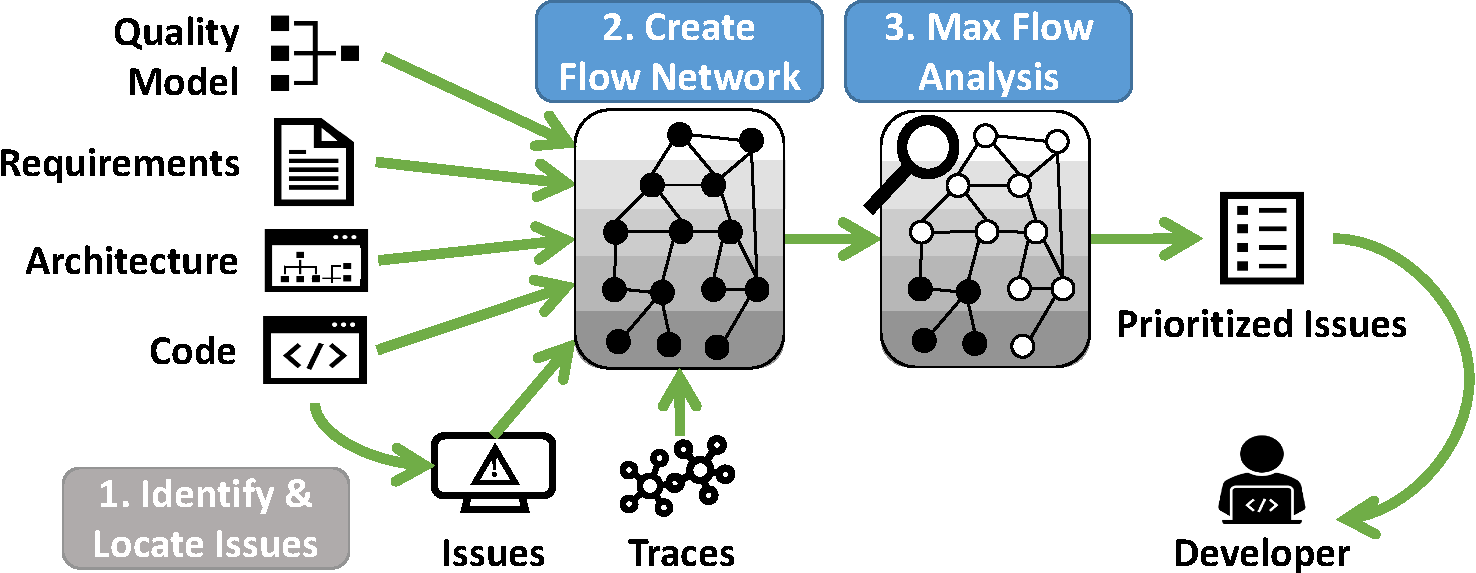
\includegraphics[width=.6\columnwidth]{figures/Gesamtschaubild-v05-KG.pdf}%width=0.8\textwidth
	\caption{Concept of the Issue Prioritization Technique}
	\label{fig:PrioApproach}
\end{figure}

\begin{enumerate}[label=\arabic*.]
    \item First, we \emph{identify and locate %security
    issues} with current static analysis tools. %, e.g., SonarQube.
%We do not propose new static analysis methods in this work but rely on state-of-the-art technology that is widely used in practice.
%%This usually results in a large list of issues.
%%It is unclear which of these issues should be addressed first as it is not clear which ones are actually security-relevant because they are located in a critical part of the implementation and can be exploited.
%Our main contributions reside in %the following
%steps 2 \& 3 (highlighted in \autoref{fig:PrioApproach}).

\item Second, we \emph{create a flow network of trace links} between the available development artifacts and these issues, thus embedding contextual knowledge into the prioritization.
To reflect the importance of different trace links, we apply capacities to them %the trace links
based on the linked artifact types and their interrelations.

%A quality model\,\cite{Deissenboek2009,Schneider2012ASQ,WAGNER2015101} is used to organize the quality goals and detail them to quality requirements. It serves as a core %element
%reference
%in security planning and prioritization and enables us to prioritize security issues in a later stage. However, our approach supports arbitrary artifacts that can be mapped to models and among which trace links exist.

\item Third, we \emph{analyze the flow network of interconnected artifacts} to calculate the security-related priorities of issues by reducing the prioritization to the \textit{maximum flow problem}\,\cite{harris1955} for each identified issue.
With this algorithm, we calculate a priority for each issue instance found by a static analysis tool, by following the trace links.
This priority reflects the connection between the issue and the project's security preferences captured in qualities, indicating the potential impact on the preferred security qualities.
\end{enumerate}

\noindent
If a static code analysis tool detects %security
issues, using \appr{}, the developer can focus on the most important issues first.
%
We do not propose new static analysis methods in this work but rely on state-of-the-art technology that is widely used in practice.
%This usually results in a large list of issues.
%It is unclear which of these issues should be addressed first as it is not clear which ones are actually security-relevant because they are located in a critical part of the implementation and can be exploited.
Our main contributions reside in %the following
steps 2 \& 3 (highlighted in \autoref{fig:PrioApproach}).
%
To this end, the contributions presented in this paper are:

\begin{itemize}
    \item The \appr{} issue prioritization technique that leverages project-specific knowledge captured in project artifacts as well as trace links and maps the issue prioritization itself to a maximum flow problem.

    %\item A domain-specific language (DSL)\,\cite{fowler2010domain,dsl} that allows arbitrary model-based artifacts to be supported in prioritization, and to tailor the prioritization based on how different artifacts are used in individual projects.

    \item Publicly available open source tool support, which comes with a domain-specific language (DSL) that allows arbitrary model-based artifacts to be supported in prioritization, and to tailor the prioritization based on how different artifacts are used in individual projects. We provide specifications written in this DSL\,\cite{fowler2010domain,dsl}
    for supporting UML models\,\cite{uml}, a program model for Java programs\,\cite{peldszus2016continuous,Peldszus2022}, as well as our own publicly available metamodels for quality models and requirements\,\cite{replication}.

    \item An evaluation of \appr{} concerning
    \begin{itemize}
        \item its effectiveness in issue prioritization in comparison to widely used state-of-the-art rule priorities,
        \item how well project specific security requirements can be considered in the prioritization based on preferences specified in quality models,
        \item the scalability of \appr{} in the context of large projects and the involved overhead for using it, and
       % \item the impact of imperfect trace links and planning artifacts on the prioritization.
    \end{itemize}

    Evaluation results show that our prioritization is closer to manual prioritization than prioritization based on SonarQube rule priorities, that project-specific preferences captured in a quality model indeed influence the issue prioritization, and that our technique scales well even for large software projects.
\end{itemize}

\noindent
	We provide practitioners and tool builders with insights on how to automatically include planning artifacts into the prioritization of issues detected by static analyzers.
	We provide researchers with first insights of how traceability affects prioritization and the means to investigate the relationship between implementation-level issues and security planning artifacts, i.e., the security design, in depth.

This work is structured as follows.
First, we give the required background in \autoref{sec:background} and introduce our prioritization technique in detail in \autoref{sec:approach}.
To this end, we first discuss different artifacts commonly created during systems development and the relations among them that could be leveraged by \appr{} in \autoref{DevArt}.
Based on these artifacts, we introduce how to extract a flow network from them in \autoref{sec:flownetwork}. We discuss how to systematically tailor the flow network construction towards potentially varying needs due to project context or the used artifacts and introduce a domain-specific language~(DSL) that allows the reusable specification of such tailoring in \autoref{sec:dsl}.
In \autoref{sec:tool} we introduce the tool support of \appr{} that is leveraged for the evaluation of \appr{}, which is presented in detail in \autoref{sec:eval}.
We close the work with a discussion in \autoref{sec:disc},
%where we consider assumptions and implications in \autoref{sec:implication} and threats to validity in \autoref{sec:threats},
related work in \autoref{sec:rw}, and a conclusion in \autoref{sec:conslusion}.